\documentclass[a4paper, 11pt]{article}

\usepackage[english]{babel}
\usepackage{titlesec}
\usepackage{listings}



\usepackage{afterpage}
\usepackage{makeidx}
\usepackage[hidelinks, breaklinks]{hyperref}
\usepackage[hyphenbreaks]{breakurl}

\usepackage[style=numeric]{biblatex}

\usepackage{caption}
\usepackage{subcaption}
\newcommand{\source}[1]{\caption*{Source: {#1}} }


\usepackage{tocloft}
\renewcommand{\cftsecleader}{\cftdotfill{\cftdotsep}}



\usepackage{cancel}

% Load the package
\usepackage{glossaries}

% Generate the glossary
\makeglossaries

\usepackage[utf8]{inputenc}
\usepackage{mathtools}

\usepackage{amsmath}

\usepackage{graphicx}
\usepackage{multicol,lipsum}


\usepackage{indentfirst}

%%%%% PACKAGES QUE EU FUI BUSCAR %%%%%

\usepackage{comment}

\usepackage{pdfpages} % Package para pdf segundo o Stack Overflow

\usepackage{color, colortbl}

\usepackage{gensymb} % Acrescentei este para conseguir ter o simbolo de degree


\usepackage{sectsty}

\sectionfont{\fontsize{12}{12}\selectfont}
\usepackage[a4paper, total={6in, 9in}]{geometry}


% CABEÇALHO E RODAPÉ

\usepackage{fancyhdr}

\pagestyle{fancy}
\fancyhf{}
\fancyhead[LE,RO]{2023/2024}
\fancyhead[RE,LO]{FEUP}
\fancyfoot[LE,RO]{\thepage}

%%%%%%%%%%%%%%%%%%%%%%%%%%%%%%%%%%%%%%%

\begin{document}

\begin{titlepage}

\begin{center}


\begin{figure}[h]
    \centering
    
\includegraphics[width=7cm, height=2.75cm]{feup}
\end{figure}
\vspace{100pt}

\LARGE{\textbf{Adversarial Search Methods for Two-Player Board Games}} \par
\large{Artificial Intelligence}

\vspace{70pt}

\Large{\textbf{Turma 10 - Grupo A1 91}} \par

\vspace{20pt}

\normalsize{
Ntsay Zacarias up202008863 \par
}


\vspace{90pt}

\large{1 de Abril de 2024}

\end{center}

\end{titlepage}

\newpage

\tableofcontents

\newpage

\section{Introduction}
The objective of this project was to explore and highlight the differences in the implementation of various adversarial search algorithms in board games. Among these, I selected the somewhat lesser-known game, \textbf{Focus}, for analysis. Focus represents a zero-sum, inherently adversarial game with a complex state space, making it an ideal candidate for the application of techniques such as MiniMax, Monte Carlo Tree Search (MCTS), and their variants. The game's deterministic nature further complements these strategies, enabling precise planning and execution of moves. My primary goal was to deepen my understanding of Focus to develop and implement effective heuristics that capitalize on the unique aspects and rule nuances of the game.

\par


\begin{figure}[htp]
    \centering
    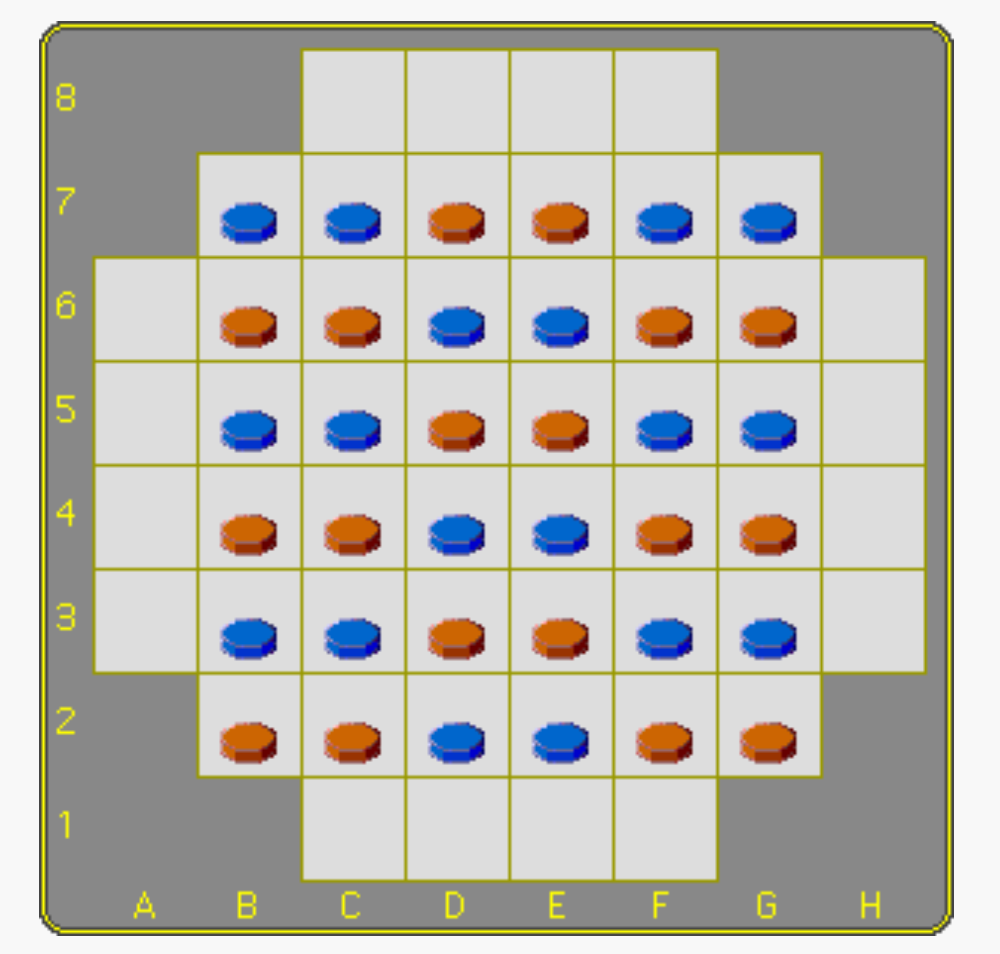
\includegraphics[width=15cm, height=12cm]{board-img}
    \caption{}
    \label{fig:Focus}
\end{figure}
\vspace{10pt}
\textcolor{gray}{
Focus is a game played on a square board with some of the corners removed.
It is an abstract strategy game in which players attempt to make moves and
capture pieces in such a manner that their opponent(s) have no moves remaining
}
\subsection{Rules}
Each player has 18 pieces, let's call each of them a \textbf{man}, and they can stack on each other, creating stacks of \textbf{men}. \par

\begin{itemize}
    \item A stack is owned by the player whose color is on top
    \item On his turn a player moves a man or a stack of men horizontally or vertically, based on the number of pieces to be moved (Stacks may be split in this process)
    \item When a stack grows over five pieces tall, the remaining men are removed from the bottom of the stack
    \begin{itemize}
        \item Men of a player's own color become 'reserves' to be re-entered into the game at a later time
        \item Pieces of the opponent's color are captured
    \end{itemize}
    \item Instead of moving a piece, a player may choose to enter one of his reserves on any square of the board, whether vacant, or occupied by a piece of either color
\end{itemize}

\subsection{Objectives (End States)}
\begin{itemize}
    \item A player wins when his opponent cannot move a piece, nor enter a reserve on
the board
\end{itemize}



\section{Related Work}

\section{Problem Formulation}
\subsection{State Representation}
A state is represented as a 2D matrix, where each cell \((i, j)\) contains a list of integers representing the stack of pieces at that position. Player 1's pieces are denoted by 1, and Player 2's pieces by 2. Non-playable cells are represented by \texttt{None}.

\subsubsection{Initial State}
The initial state is the board setup with each player's pieces in their starting positions, and corners of the board removed (set to \texttt{None}).

\subsubsection{Operators}

\paragraph{Move}
\begin{itemize}
    \item \textbf{Preconditions}: The source cell contains a stack, the move is within board limits, and it adheres to the game's movement rules.
    \item \textbf{Effect}: The stack is moved or split, capturing or merging with stacks at the destination.
    \item \textbf{Cost}: 1
\end{itemize}

\paragraph{Enter Reserve}
\begin{itemize}
    \item \textbf{Preconditions}: The player has at least one piece in reserve.
    \item \textbf{Effect}: A piece from the reserve is placed on any cell on the board, starting or adding to a stack.
    \item \textbf{Cost}: 1
\end{itemize}

\paragraph{Capture}
\begin{itemize}
    \item \textbf{Preconditions}: A stack grows over five pieces tall after a move.
    \item \textbf{Effect}: Pieces exceeding the stack limit are removed. Own pieces become reserves; opponent's pieces are captured.
    \item \textbf{Cost}: Implicit in the move cost.
\end{itemize}

\subsubsection{Objective Test}
The objective is to reach a state where the opponent cannot make a valid move or enter a reserve, thereby winning the game.



\section{Implementation}

\end{document}



https://www.overleaf.com/project/6602e6c5ac891a2f1c58034a